\chapter{Estrutura e funcionamento\label{cap:detalhamento-projeto}}

    \section{Processo de instalação\label{sec:processo-instalacao}}
        O \emph{Framework Lothus\{PHP\}} permite ao desenvolvedor a possibilidade de escolha entre dois níves de aplicação. O primeiro nível permite a instalação do \emph{Framework} da forma mais simples, instalando utilitário focados em um desenvolvimento direcionado ao backend do projeto, integrando facilidade a troca de informações com o banco de dados, desenvolvimento através do MVC, URLs amigáves e sistemas de templates.

        Essa instalação é feita através do repositório remoto \emph{Github}, que se encontra no seguinte endereço online:

        \emph{https://github.com/guilouro/Lothus-PHP}

        O Github permite duas formas de download de um projeto: fazendo o downloand de um arquivo comprimido em .zip diretamente do site ou utilizando um sistema de versionamento de arquivos para fazer o clone do mesmo. Neste projetos iremos usar o \emph{Git} como sistema de versionamento. Para fazer o clone utilizando o git executamos a seguinte linha de comando no terminal Unix ou cmd Windows:

        \textbf{\$ git clone https://github.com/guilouro/Lothus-PHP.git}

        Ao executar essa linha de comando, uma nova pasta será criada com o nome de Lothus-PHP. Dentro desta nova pasta estará todo o projeto para iniciar o desenvolvimento utilizando o \emph{Framework Lothus\{PHP\}}. O próximo capítulo será responsável pela apresentação das pastas existentes dentro do projeto.



    \section{Estrutura de pastas e arquivos\label{sec:estrutura-pastas}}
        Neste capítulo será apresentado a estrutura de pastas do \emph{Framework Lothus\{PHP\}} juntamente com o processo de criação e funcionamento de cada etapa.

        Ao clonar o projeto utilizando o git, como visto no capítulo anterior, será gerada uma estrutura de pastas dentro da pasta Lothus-PHP.

        \begin{figure}[!htb]
            \centering
            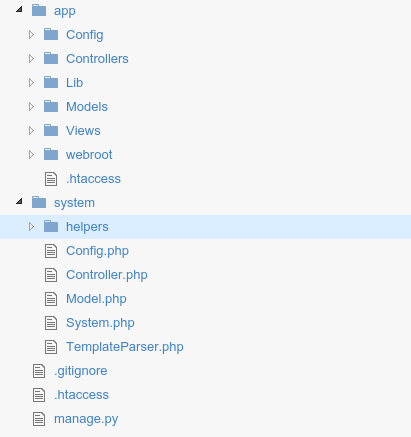
\includegraphics[scale=0.8]{pastas.jpg}
            \caption{\small Estrutura do projeto}
            \label{cap:sass}
        \end{figure}

        Neste primeiro momento já ocorre uma pequena divisão do projeto onde a pasta \emph{app} é responsável por gerenciar a aplicação e a pasta \emph{system} responsável pelo \emph{core}, ou seja, gerenciamento interno do framework. Em sua raiz existe, além dessas duas pastas, três importantes arquivos para o projeto, que são:

        \begin{itemize}
            \item \textbf{.gitignore}: Um arquivo que faz parte da configuração do git e é responsável por guardar, linha por linha, todos os arquivos ou pastas serão ignorados pelo git no momento de fazer o versionamento do projeto. Isso evita o acumulo de arquivos desnecessários, que são gerados automaticamente, no pacote de instalação do Framework.

            \item \textbf{.htaccess}: Arquivo que é lido antes do index.php e tem a responsabilidade de criar a rota inicial do projeto, fazendo o direcionamento para o arquivo correto na inicialização do sistema.

            \begin{figure}[!htb]
                \centering
                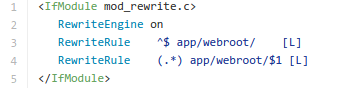
\includegraphics[scale=0.8]{htaccess1.jpg}
                \caption{\small Estrutura do htaccess na raiz do projeto}
                \label{cap:sass}
            \end{figure}

            \item \textbf{manage.py}: Trata-se de um script de linha de comando capaz de gerar novos arquivos baseados na arquitetura de funcionamento do \emph{Framework}. A imagem abaixo ilustra o uso básico da ferramenta.

            \begin{figure}[!htb]
                \centering
                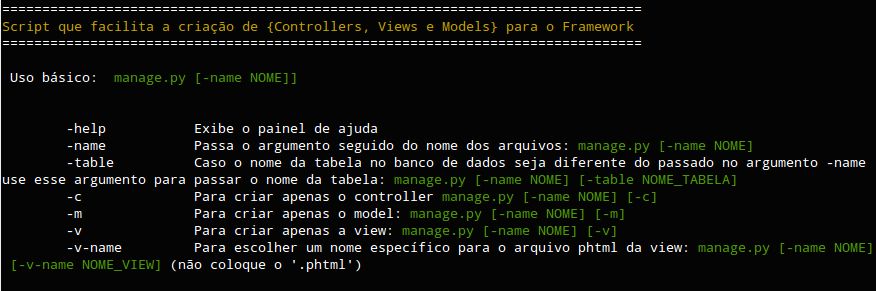
\includegraphics[scale=0.5]{manage.jpg}
                \caption{\small Regras para uso básico do manage.py}
                \label{cap:sass}
            \end{figure}


        \end{itemize}

    \section{Sistema\label{sec:system-core}}

        O Framework recebe um primeiro nível de divisão no processo de criação do mesmo, que é a divisão do Sistema par a Aplicação o sistema fica todo centralizado na pasta \emph{system}, e é onde contém o motor do \emph{Framework}, nele estão todas as classes responsáveis pelas regras de funcionamento do projeto, tanto nas requisições HTTP, passando por padronização de Controllers, Views até chegar ao relacionamento com o banco de dados. Todas essas funcionalidades estão divididas entre classes e arquivos que serão detalhados ao longo deste capítulo.

    \begin{figure}[!htb]
        \centering
        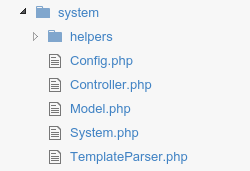
\includegraphics[scale=0.6]{system-path.jpg}
        \caption{\small Estrutura interna da pasta system}
        \label{cap:sass}
    \end{figure}



        \subsection{Config\label{sub:system-config}}

            A Classe \emph{Config} é responsável pela configuração inicial de qualquer projeto que faz uso do \emph{Lothus\{PHP\}}. Ela tem a responsabilidade de definir qual \emph{View} será iniciada ao acessar o link do sistema e também se responsabiliza em definir se será exibido ou não um \emph{debug} para o desenvolvedor.

            \emph{}

            O arquivo \emph{Config.php} possui a seguinte estrutura:

            \emph{}

\begin{lstlisting}
class Config {
    public  $_Index = "home";
    private $error = TRUE;

    protected function ERROR($pag){}
}
\end{lstlisting}



        \begin{itemize}
            \item\textbf{\$\_Index}: É uma variável \textbf{pública} que recebe, como string, o nome do \emph{Controller} padrão a ser requisitado pelo sistema no caso de a URL não ter, explicitamente, este valor.

            \item\textbf{\$error}: Trata-se de uma \textbf{privada} váriavel booleana, que funciona como uma chave para exibir um erro para o desenvolvedor ou direcionar o usuário para uma página 404, no momento em que for acessada alguma página inexistente. No caso de \textbf{\$error = TRUE} será exibido uma mensagem de alerta ao desenvolvedor sobre alguma falha nos padrões do \emph{Framework}. Caso \textbf{\$error = FALSE} o usuário será redirecionado para uma página de \emph{erro 404}

            \item\textbf{ERROR(\$pag)}: É um método protegido, que recebe como parâmetro o nome da página que não foi encontrada no sistema. Sua funcionalidade é, inicialmente, verificar se a variável \textbf{\$error} é \textbf{TRUE} \emph{(Verdadeiro)} ou \textbf{FALSE} \emph{(False)}, para posteriormente, direcionar o usuário para a página de erro padrão do sistema ou exibir uma mensagem dizendo se o erro foi causado pela falta de um \emph{Controller} ou de uma \emph{Action} para o sistema.
        \end{itemize}

        \emph{}

        \emph{}

        A lógica de programação aplicada a este métdo é a seguinte:

        \emph{}

\begin{lstlisting}
protected function ERROR($pag) {
    if($this->error) {
        /* Erro em Controller ou Action */
    } else {
        /* Redirecionamento */
    }
}
\end{lstlisting}

        \subsection{Url amigável e o padrão MVC\label{sub:url-amigavel}}

        \subsection{System\label{sub:system-sis}}

        \subsection{Helpers\label{sub:system-helper}}



        \subsection{Controller\label{sub:system-controller}}

        \subsection{Model\label{sub:system-model}}

        \subsection{Template\label{sub:system-template}}


    \section{Aplicação\label{sec:app}}

        falar do htaccess

        \subsection{Config\label{sec:app-config}}

        \subsection{Model\label{sec:app-model}}

        \subsection{View\label{sec:app-view}}

        \subsection{Controller\label{sec:app-controller}}

        \subsection{Lib\label{sec:app-lib}}

        \subsection{webroot\label{sec:app-lib}}


        \subsection{Controller\label{sec:app-controller}}


    \section{Divisão Backend - frontend\label{sec:back-front}}


        \subsection{Comandos do Grunt\label{sub:comandos-grunt}}

    \section{System\label{sec:estrutura-pastas}}

    \section{Model\label{sec:estrutura-pastas}}

    \section{View\label{sec:estrutura-pastas}}

    \section{View\label{sec:estrutura-pastas}}

    \section{Template\label{sec:estrutura-pastas}}
